\documentclass[openright]{normas-utf-tex} %openright = o capitulo comeca sempre em paginas impares

\special{papersize=210mm,297mm}

\usepackage[alf,abnt-emphasize=bf,bibjustif,recuo=0cm, abnt-etal-cite=2, abnt-etal-list=99]{abntcite} %configuracao correta das referencias bibliograficas.

\usepackage[brazil]{babel} % pacote portugues brasileiro
\usepackage[utf8]{inputenc} % pacote para acentuacao direta
\usepackage{amsmath,amsfonts,amssymb} % pacote matematico
\usepackage{graphicx} % pacote grafico
\usepackage{times} % fonte times
\usepackage[final]{pdfpages} % adicao da ata

\instituicao{Universidade Tecnológica Federal do Paraná} % nome da instituicao
\programa{Programa de Pós-graduação em Engenharia Elétrica e Informática Industrial} % nome do programa
\area{Informática Industrial} % [Engenharia Biom\'edica] ou [Inform\'atica Industrial] ou [Telem\'atica]

\documento{Dissertação} % [Disserta\c{c}\~ao] ou [Tese]
\nivel{Mestrado} % [Mestrado] ou [Doutorado]
\titulacao{Mestre} % [Mestre] ou [Doutor]

\titulo{{Título em português}} % titulo do trabalho em portugues
\title{\MakeUppercase{Title in English}} % titulo do trabalho em ingles

\autor{Nome do Autor} % autor do trabalho
\cita{SOBRENOME, Nome} % sobrenome (maiusculas), nome do autor do trabalho

\palavraschave{Palavra-chave 1, Palavra-chave 2, ...} % palavras-chave do trabalho
\keywords{Keyword 1, Keyword 2, ...} % palavras-chave do trabalho em ingles

\comentario{\UTFPRdocumentodata\ apresentada ao \UTFPRprogramadata\ da \ABNTinstituicaodata\ como requisito parcial para obtenção do grau de ``\UTFPRtitulacaodata\ em Ciências'' -- Área de Concentração: \UTFPRareadata.}

\orientador{Nome do Orientador} 
\local{Curitiba} % cidade
\data{\the\year} % ano automatico

% desativa hifenizacao mantendo o texto justificado.
% thanks to Emilio C. G. Wille
\tolerance=1
\emergencystretch=\maxdimen
\hyphenpenalty=10000
\hbadness=10000
\sloppy

%---------- Inicio do Documento ----------
\begin{document}

\capa % geracao automatica da capa
\folhaderosto % geracao automatica da folha de rosto

% Lembre-se de que a ficha catalografica eh impressa no verso da folha de rosto
% Ficha catalografica
\fichacatpum{T137}
\fichacatautor{Sobrenome, Nome}
\fichacatpgbib{\pageref{bibstart}-\pageref{bibend}}
\fichacatpalcha{1. Teoria do controle. 2. Redes de comutação. 3. TCP/IP (Protocolo de rede de computação), ...}
\fichacatpdois{CDD (22. ed.) 621.3}
\fichacatbib{Biblioteca xxxxxx}
\fichacat

% insercao da ATA
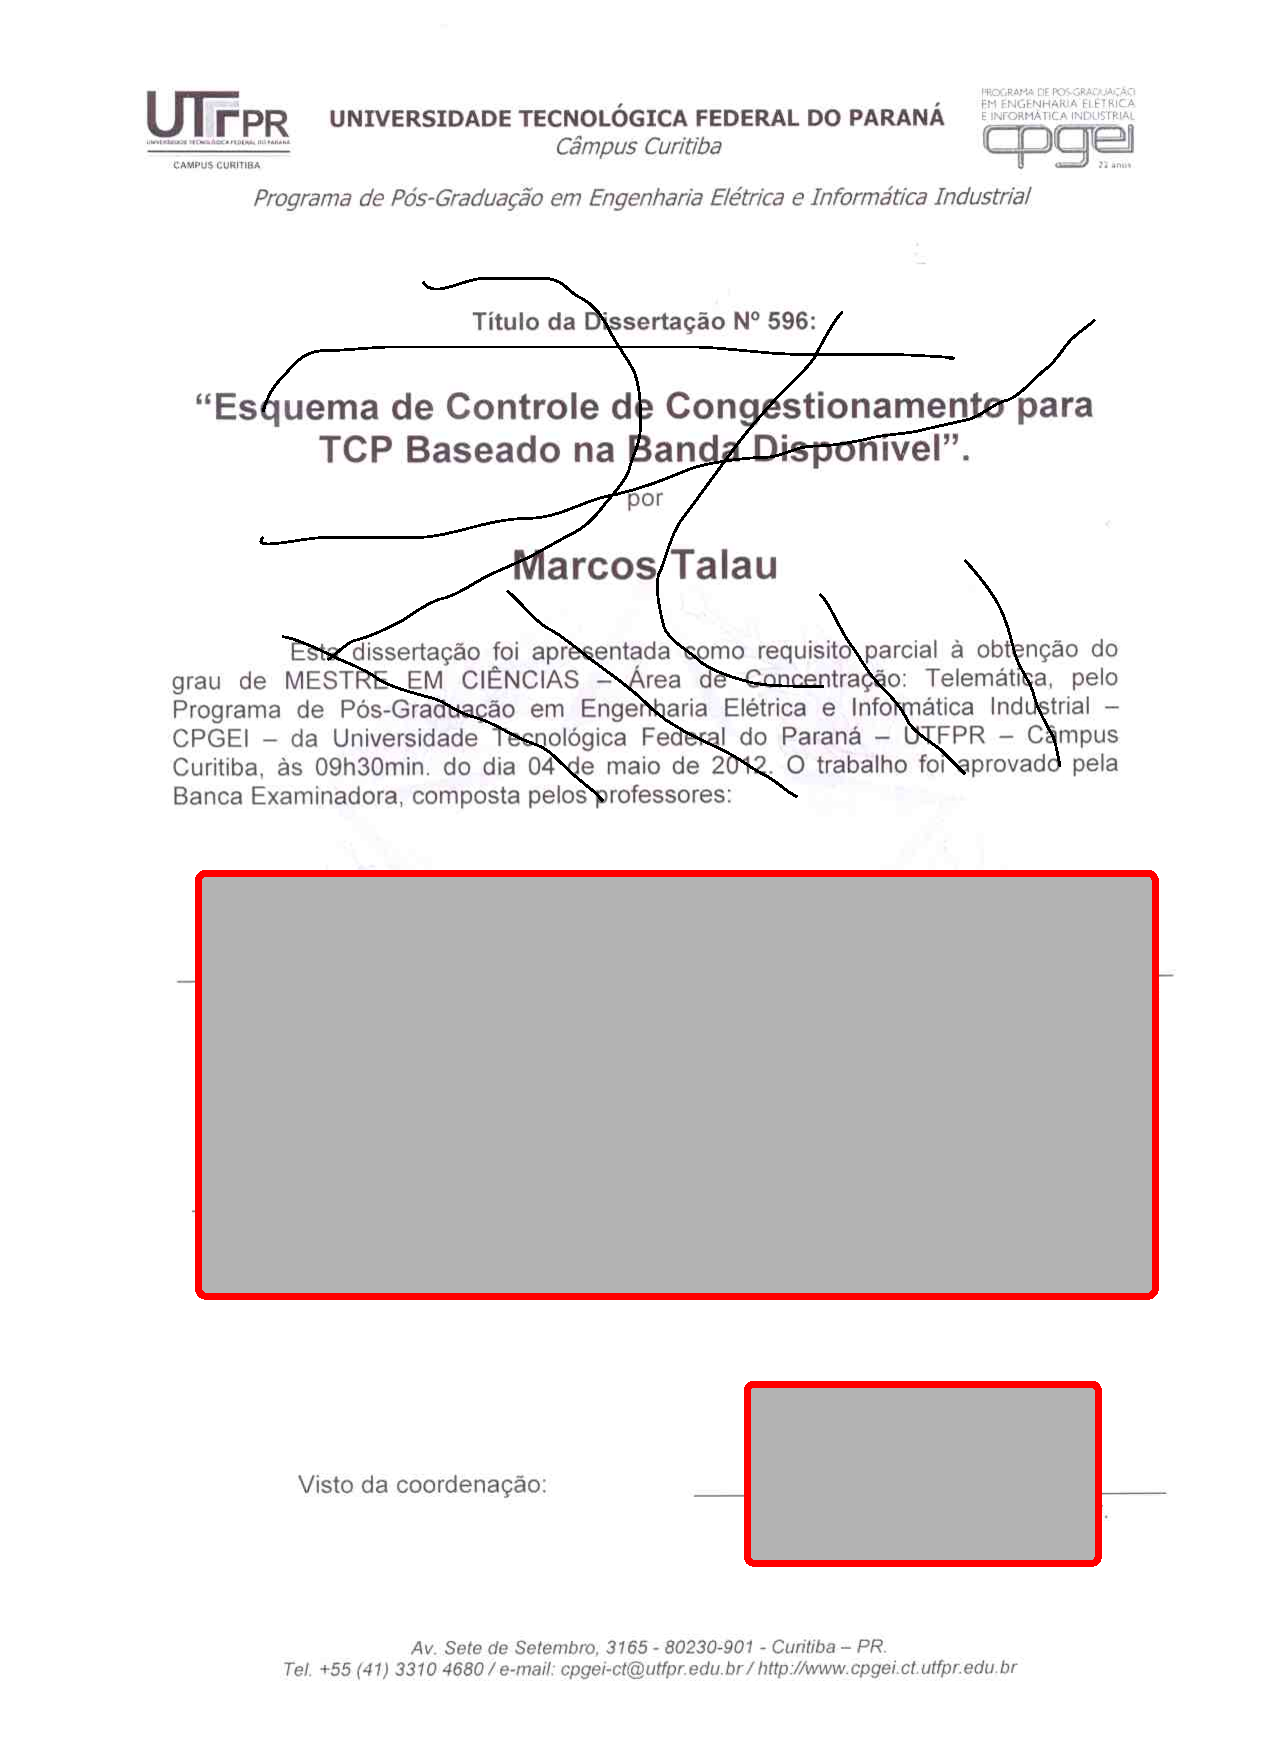
\includepdf{ata.pdf}

% dedicatoria
\begin{dedicatoria}
Texto da dedicat\'oria.
\end{dedicatoria}

% agradecimentos (opcional)
\begin{agradecimentos}
Texto dos agradecimentos.
\end{agradecimentos}

% epigrafe (opcional)
\begin{epigrafe}
Texto da ep\'igrafe.
\end{epigrafe}

%resumo
\begin{resumo}
Texto do resumo (m\'aximo de 500 palavras).
\end{resumo}

%abstract
\begin{abstract}
Abstract text (maximum of 500 words).
\end{abstract}

% listas (opcionais, mas recomenda-se a partir de 5 elementos)
\listadefiguras % geracao automatica da lista de figuras
\listadetabelas % geracao automatica da lista de tabelas
\listadequadros % adivinhe :)
\listadesiglas % geracao automatica da lista de siglas
\listadesimbolos % geracao automatica da lista de simbolos

% sumario
\sumario % geracao automatica do sumario

\setcounter{page}{12}

%---------- Primeiro Capitulo ----------
\chapter{Introdução}

	Diversas pessoas são submetidas a algum tipo de risco na execução de atividades profissionais. Trabalhos como de eletricistas, bombeiros, área petroquímica, serviços de telecomunicações e de transporte (motoristas de ônibus e de carro) são apenas alguns em que onde profissionais são expostos a condições de risco.

Acidentes em situações assim ocorrem pelos mais diversos motivos. Investigar as cadeias de causalidade que resultam nessas situações pode trazer um entendimento de como lidar com essas circunstâncias. Consequentemente, isso traz um potencial para diminuir o número de acidentes. A computação é uma ciência que apresenta um grande potencial de contribuição para a resolução desse problema. Isso envolve criar representações que descrevam atividades com riscos de acidentes e que permitam realizar raciocínios sobre essas relações de causalidade.

Algo que exemplifica essa situação são as atividades praticadas por profissionais que trabalham com eletricidade em linha viva. Isso, pois esses trabalhadores realizam procedimentos de manutenção em componentes, estruturas e equipamentos elétricos energizados que demandam fluxo de potência elétrica (ex. transformadores, condutores). A particularidade nos processos de linha viva consiste no fato de que esses equipamentos e estruturas se mantêm energizados durante a ação dos profissionais. Essa situação expõem esses profissionais a perigos de acidentes com eletricidade causando mortes ou ferimentos extremamente sérios com danos permanentes a vida dos acidentados.  
	
	\section{Motivação}	
	
		Uma das motivações desse estudo reside em obter uma compreensão do problema em voga por meio de um modelo conceitual concebido com base em dois fatores. O primeiro fator consiste numa averiguação de modelos computacionais que são aplicados em sistemas multiagentes (inclusive os normativos). O segundo fator consiste em averiguar um dado estudo de caso a fim de abstrair estruturas conceituais que possam ser do interesse dessa pesquisa.

Uma outra motivação desse estudo consiste em averiguar como o modelo conceitual resultante pode ser vinculado a arcabouços e modelos computacionais que fazem parte do \textit{mainframe} acadêmico no campo da computação em sistemas multiagentes normativos.

A motivação desse estudo, portanto, reside em explorar e entender a problemática atrelada a cenários de acidentes e riscos com a finalidade de avaliar com clareza as possibilidades existentes dentro do contexto computacional.
	
	\section{Objetivos}

		Essa subseção tem a finalidade de apresentar o objetivo geral bem como os objetivos específicos dessa pesquisa. 

		\subsection{Objetivo Geral}

			Sintetizar, construir e avaliar, por intermédio de observações, de análises de documentos técnicos, de análises de modelos computacionais e de entrevista com profissionais da área, um modelo conceitual que define os conceitos e as relações para representar os cenários de ambientes de atividades, bem como os respectivos acidentes que podem acontecer, em que a validação ocorre por verificar se os raciocínios (para um dado estudo de caso do setor de energia elétrica) resultantes desse modelo são correspondentes com a realidade a fim de levantar um entendimento formal do problema para a comunidade acadêmica no que tange a que tipo de representação computacional é mais apropriada para determinado contexto. 
			
		\subsection{Objetivos Específicos}

			\begin{itemize}
    \item Identificar os pontos essenciais que devem fazer parte da estrutura do modelo em relação aos riscos e consequências (acidentes) para os atores e atividades (continuidade), que sejam relevantes na prática da atividade de manutenção, em caso de falha na operação. 
    \item Construir um modelo conceitual que implementável computacionalmente e que produza as inferências que respondam às questões definidas como essenciais.
    \item Validar o modelo por aplica-lo a um dado estudo de caso a fim de averiguar se os raciocínios produzidos nessa situação estão de acordo com a realidade.  
    \item Analisar modelos computacionais em relação ao modelo conceitual desse estudo a fim de ter um levantamento formal do estado do problema.
\end{itemize}


%---------- Segundo Capitulo ----------

\chapter{Fundamentação Teórica}
\label{chap:fundteoric}

	\section{Agentes}

		Não existe uma definição universal para tratar o conceito de agente sendo que esse tópico se encontra em meio a debates e controvérsias. Contudo, existe um entendimento generalizado de que 
um comportamento \textit{autonomo} é o cerne de noção que se tem por agente \cite{whatisagent}.  Apesar disso, a construção de um modelo computacional não pode ser feito sem uma definição. Assim sendo, nesse texto um agente é
 um sistema computacional que está situado em um dado ambiente e que apresenta comportamento autonomo \cite{definitionagent} \cite{whatisagent}. Não apenas isso, mas um agente faz uso
 so seu comportamento autonomo com o propósito de atingir objetivos que a ele é designado \cite{definitionagent} \cite{whatisagent}.

Dentro do contexto presente na definição de agentes, um ambiente apresenta as seguintes propriedades \cite{artificialinteligencemodermapproach} \cite{whatisagent}; 
\begin{itemize}
    \item \textit{Acessibilidade vs Inacessibilidade}; Um ambiente acessível é aquele onde um agente consegue ter informações claras, precisas e atualizadas no que tange a característica do ambiente.
    \item \textit{Determinístico vs Não-Determinístico}; Um comportamento determinístico é aquele onde uma ação possui um efeito claro e garantido, sem incertezas sobre o estado que irá resultar.
    \item \textit{Episódico vs Não-Episódico}; Um ambiente tende a ser o mais episódico possível tanto quando o desempenho do agente estiver associado a um episódio discreto e específico no ambiente.
    \item \textit{Estático vs Dinâmico}; Um ambiente é estático se não houver outros processos em parapelo aos eventos associados ao agente.
    \item \textit{Discreto vs Contínuo}; Um ambiente é discreto se existe um número finito de ações e percepções. 
\end{itemize}

Outro aspecto a ser considerado em um agente implica o comportamento autonomo. Uma entidade que possui essa natureza tem a capacidade agir por sí mesmo. Essa entidade não precisa de nenhuma outra entidade externa 
(ex. ser humano) para realizar decisões \cite{whatisagent} \cite{definitionagent}.

Há uma série de exemplos que se enquadram dentro dessa deinição. Sistemas de controle se enquadram nesses exemplos. Um \textit{termostato} é um sistema de controle que está em um dado ambiente 
(como um quarto ou uma sala) \cite{whatisagent}, gera dois sinais de saída (um desses sinais indica que a temperatura está baixa demais (ou alta demais dependendo da aplicação) e o outro sinal
demonstra que a temperatura está no nível aceitável). O termostato tem o seu comportamento autonomo baseado em duas regras \cite{whatisagent}:

\begin{itemize}
    \item Se a temperatura estiver abaixo (ou acima) do nível de temperatura definido, então ligar o atuador.
    \item Se a temperatura estiver dentro do nível estabelecido, então desligar o atuador.
\end{itemize}

Outro exemplo de agentes consiste nos programas \textit{Daemons} em sistemas \textit{UNIX}. Esses algoritmos trabalham em segundo plano e monitoram um dado ambiente de \textit{software}. Com base
em certas regras, na ocorrência de um dado evento no ambiente, esses programas realizam uma dada atuação \cite{whatisagent}.   

Os exemplos presentes neste texto são apropriados dentro do conceito de agentes. Contudo, esses exemplos não ase equandram dentro da denição de agentes inteligentes \cite{whatisagent}. Uma entidade que se enquadra
dentro das caracterísiticas de um agente inteligente deve necessariamente respeitar a definição já apresenta e deve apresentar as seguintes propriedades; reatividade (capaz de perceber as mudanças
que ocorrem no ambiente e responder a delas de maneira apropriada no que condiz aos objetivos do agente), pro-atividade (apresenta comportamento orientado a objetivos sendo que o agente toma as decisões
a fim de satisfazer os objetivos em interesse) e habilidades sociais (capacidade de interagir com outros agentes (e possivelmente humanos) a fim de poder satisfazer os próprios objetivos) \cite{whatisagent} \cite{artificialinteligencemodermapproach}.

Os agentes podem ser definidos em categorias. Um desses são agentes puramente reativos. Esses agentes tomam decisões considerando apenas informações que estão no instante presente. Por consequência, 
o comportamento deles ocorre por respostas diretas ao ambiente \cite{whatisagent}. 

Outra categoria de agentes são aqueles que possuem estados. Essas entidades possum uma dada estrutura de dados internar que são considerados quando agente toma uma uma certa decisão \cite{whatisagent}.

Uma outra maneira de analisar os agentes se dá por meio das arquiteturas e modelos disponiveis para representar os agentes (tomada de decisão, estado interno). Para o propósito do estudo que está
sendo apresentando neste texto, é o suficiente considerar de forma sucinta quatros dessas arquiteturas. A primeira consiste nos agentes baseados em lógica onde os agentes realizam deduções lógicas
para tomar uma decisão \cite{logicagent}, a segunda arquitetura consiste nos agentes reativos que tomam decisões com base em um dado mapeamento de uma certa situação em uma dada ação \cite{reactiveagent}, a terceira arquitetura é \textit{BDI}
cuja decisão ocorrem da manipulação de estruturas de dados que representam crenças, desejos e intenções do agente \cite{bdi} e a quarta arquitetura consiste em uma estrutura em camadas onde a tomada de decisão
acontecem por intermédio de diversas camadas abstração a cerca do ambiente \cite{layeragent} \cite{whatisagent}.  

	\section{Sociedades Multiagentes}

		Um sistema multiagente(SMA) organizado é aquel constituido por agentes autonomos que interagem visando um propósito em comum tendo como consequência um comportamento global \cite{mosieframework} 
\cite{organiationofmultiagentsystem}. Assim sendo, uma organização com essas características deve ser capaz de manifestar conhecimento em comum, cultura, memória, história, distribuição de atividades 
e a capaciade de distinguir um  agente em espeçifico \cite{organiationofmultiagentsystem}. Deste fato é possível identificar o fenômeno "supra-individual" que implica em um comportamento que existe
além dos comportamentos e atributos particulares no que diz respeito as entidades constituintes do sistemas. 

Uma organização de um sistema multiagente deve conter relações sociais no que tange a agentes, institutos e grupos sociais \cite{organiationofmultiagentsystem}. Ainda sobre isso, uma organização 
\textit{SMA} deve apresentar uma \textit{extensão de um espaço abstrato}. Isso implica uma representação dos seguintes conceitos; estrutra espacial, estrutura temporal, símbolos, semântica e 
capacidade de dedução. Há organizações que não se enquadram em todas essas restrições, contudo são suficientes para tratar o problema dentro de uma perspectiva computacional \cite{organiationofmultiagentsystem}.

\subsection{Conceitos Gerais de uma Organização SMA}

A finalidade desta subseção consiste trabalhar com uma maior riqueza de detalhes todos os conceitos que constituem a ideia de uma organiozação de um sistema multiagente.  
  
\textbf{Divisão em tipos de atividades:} Uma organização não é uniformemente estruturada. Isso, pois as atividades são distribuidas de forma desigual entre as diferentes entidades.
Dentro do ponto de vista fenomenologico as atividades são sujeitas a classificação e ocorrem com diferentes frequências e em diferentes regiões dentro das definições espaciais da organização \cite{organiationofmultiagentsystem}.

\textbf{Integração:} Dentro de uma organização ocorre a presenção de interdependência entre diferentes espaços de ativiades. Essas, por sua vez, estão relacionadas em uma estrutura única definida
dentro de um contexto alinhado e integrado \cite{organiationofmultiagentsystem}.

\textbf{Composição} Uma organnização é composta por elementos menores. No caso dos multiagentes, os elementos atomicos que estruturam a organização são os agentes \cite{organiationofmultiagentsystem}.

\textbf{Estabilidade/Flexibilidade:} Uma organização apresenta padrões de atividades. Esses padrões possum cateristicas que podem ser enquadradas em dois aspectos; estaveis e flexiveis. 
No que tange as características estaveis, essas são constituidas por elementos/processos que definem o padrão em sí mesmo. Em constraste com isso um comportamento flexível acontece quando o 
sistema é submetido a situações incomuns \cite{organiationofmultiagentsystem} \textbf{?}.

\textbf{Coordenação:} Todo sistema é dependente de algum dado recurso. Assim sendo, se faz necessário que esse recurso seja utilizado de forma inteligente a fim de que possa se manter ao longo 
do tempo. Para que isso, se faz necessário que a organização se comporte como uma amplificadora de recursos a fim de que as estruturas operacionais tenham um comportamente cada vez mais organizado 
\cite{selforganization}, \cite{selforganizatioenvoriment}, \cite{defintionselforganization}, \cite{organiationofmultiagentsystem}. Ainda  



\cite{multiagentsystemmodernapproach}
\cite{multiagentsystemwhatis}
\cite{organiationofmultiagentsystem}
\cite{amodelmultiagentsystemdynamicrelationship}
\cite{mosieframework}
\cite{modelingsocialactionforaiagents}
\begin{itemize}
    \item Apresentar definições de SMA
    \item Aprestar conceito de objetivo
    \item Apresentar conceito de papel
    \item Apresentar os conceitos de relações deonticas
\end{itemize}

	\section{Normas}

		Quando se trata de normas em sistemas multiagentes é de crucial importância definir claramente este termo. Isso se deve ao fato de que há diversos estudos que tratam o conceito de norma sobre perspectivas diferentes. Por exemplo, os estudos \cite{formalizeagent} \cite{formalizeagent2} apresentam normas, em sistemas multiagentes, para representar a presença de sociedades, institutos e organizações. Há estudos que tratam normas como maneiras dos agentes trabalharem de forma coordenada com propósito de cumprir um objetivo global e também como uma maneira de obedecer as autoridades do sistema \cite{modelingnormsforautnomousagent} \cite{amodelmultiagentsystemdynamicrelationship}. No \textit{MOISE+} normas são tratadas sobre a ótica da lógica deôntica e é usada para especificar os agentes com dado papel no que condiz com as suas obrigações em relação as missões \cite{moiseframework} \cite{moiseframeworktwo}.

O estudo \cite{dastaniframework} apresenta uma linguagem formal para especificar sistemas multiagentes normativos. Essa linguagem contem os conceitos de normas que são os mesmos usados neste texto. A figura \ref{descreveprograma} apresenta a linguagem em notação EBNF \cite{dastaniframework}.

\begin{figure}[H]
  \centering
  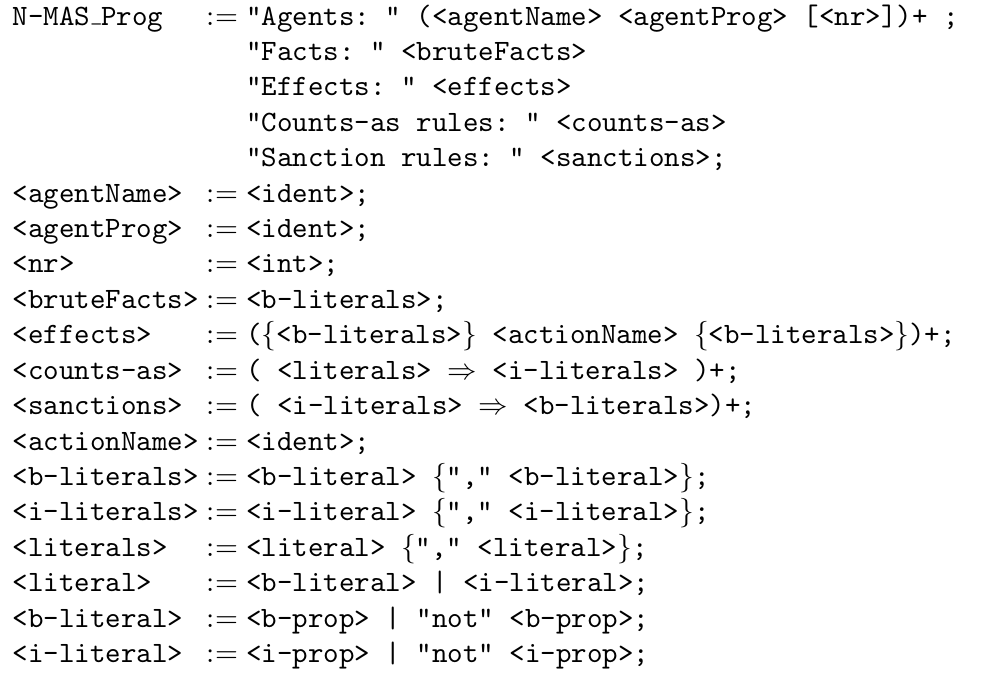
\includegraphics[width=0.8\linewidth]{figure/masprogram.png} 
  \caption{Linguagem para descrever um programa de multiagentes normativos com a possibilidade de violações e sanções na notação EBNF segundo o texto \cite{dastaniframework}. Nesta notação, $<ident>$ é usado para denotar uma \textit{string} e $<int>$ inteiros. Os termos $<b-prop>$ e $<i-prop>$ são usados para designar dois tipos de conjuntos de proposições que são disjuntos entre si}
  \label{descreveprograma}
\end{figure}

Os \textit{Facts} implementados em forma de \textit{brute facts} definem os estados iniciais do sistema dentro de um ambiente compartilhado por todos os agentes. O termo \textit{Effects}, implementado por meio de $effects$ define como se dá a transição de estados do sistema. A tag $<actionName>$ representa os eventos que geram transição dos estados. Uma norma, portanto, é definida em termos de \textit{Counts\_as rules}. O termo $<counts-as>$ aponta para transição entre $<literals>$ e $<i-literals>$. Isso representa os fatos que resultam em violações. Portanto, em \cite{dastaniframework} as normas são descritas por intermédio de suas violações. Violação, dentro deste contexto, é dado como o descumprimento da norma 
\cite{ontologynormative}.

O termo \textit{Sanction Rules} aponta para $<sanctions>$ e esses, por sua vez, para a transição entre $<i-literals>$ e $<b-literals>$ sendo que esses $<i-literals>$ advêm de \textit{Counts\_as Rules}. Assim sendo, \textit{Sanction Rules} define as consequências da violação. Essas consequências denotam caráter negativo ao agente tendo como foco uma natureza de ordem punitiva \cite{dastaniframework}. 

A figura \ref{exemploprograma} apresenta um programa escrito nessa linguagem. 

\begin{figure}[H]
  \centering
  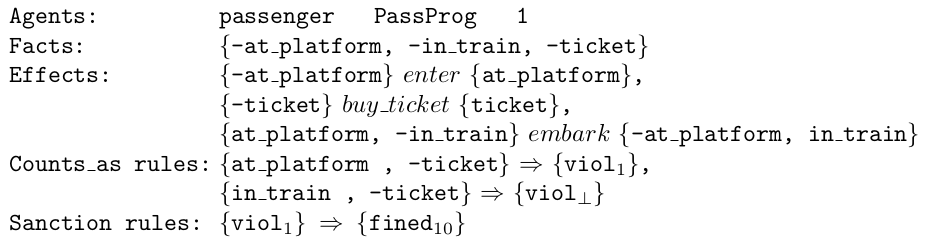
\includegraphics[width=0.8\linewidth]{figure/programdastani.png} 
  \caption{Um programa descrito na linguagem proposta neste estudo onde um agente representa um passageiro em uma estação de trem que pode entrar com ou sem um \textit{ticket} na plataforma e no trem \cite{dastaniframework}.}
  \label{exemploprograma}
\end{figure}

Esse programa contem um agente chamado de \textit{passenger} (especificações desse agente são detalhadas com maior rigor em \textit{PassProg}). Os \textit{Facts} deste programa são \textit{-at\_plataform} (agente não está na plataforma), \textit{-in\_train} (agente não está no trem) e \textit{-in\_ticket} (agente não possui o \textit{-in\_ticket}). As regras de \textit{Effects} apresentam dois $<actionName>$. O primeiro é denominado por \textit{enter} que tem por finalidade alternar entre os estados \textit{-at\_plataform} e \textit{at\_plataform}, 
ou seja, é uma ação onde o agente muda o estado de não está na plataforma para está na plataforma. O segundo estado é o \textit{buy\_ticket} que gera a transição entre os fatos \textit{-ticket} para \textit{ticket}, ou seja - na ocorrência \textit{buy\_ticket} o agente passa a ter um \textit{ticket} \cite{dastaniframework}.

O programa especifica duas regras em \textit{Counts\_as rules}. A primeira regra denota a ocorrência de uma violação para um agente que entra numa plataforma sem um \textit{ticket}. A segunda regra define que uma violação que acontece para o caso de um agente entrar em um trem sem um \textit{ticket} \cite{dastaniframework}.

O programa também define uma regra para \textit{Sanction rules}. Essa regra se aplica a $viol_1$, que - se verdade - então resulta no fato $fined_{10}$, cuja semântica denota um pagamento no valor de 10 unidades de moeda \cite{dastaniframework}.  

	\section{Sanções}

		\input{estrutura/fundamentacaoteorica/sancoes.tex}

	\section{Violações}

		\input{estrutura/fundamentacaoteorica/violacoes.tex}

	\section{Riscos}

		O primeiro estudo teórico sobre acidentes de trabalho se da no texto \cite{riskoldschool}. Essa pesquisa conclui que os erros em industria não podem ser definidos apenas nas falhas de 
humanos, mas sim como consequência de um comportamento global da instituição. Ainda dentro deste âmbito, esse comportamento advêm de uma forte pressão tendo em vista eficiência e otimização dos processos de produção \cite{riskoldschool} \cite{safety}.

Com base neste entendimento, o estudo \cite{safety} apresenta um arcabouço a fim de identificar as redes de causalidade que resultam em acidentes de trabalho. Assim sendo, a gestão de 
segurança se dá com base nos seguintes fatores; 
\begin{itemize}
    \item Políticas; \textit{leis, diretrizes, padrões e regras}
    \item Corporativo; \textit{regras, estratégias, politicas internas, gerenciamento}
    \item Projeto de Equipamentos de Trabalho; \textit{especificação, integração de segurança}
\end{itemize}

O item Política é mais relevante que os itens Corporativo e Projeto de Equipamentos de Trabalho. Esses dois últimos apresentam a mesma importância para uma estrutura de prevenção de acidentes 
bem sucedida. 

A primeira análise a ser feita diz respeito ao nível Corporativo-Projeto de Equipamentos de Trabalho. Muitas vezes a equipe adota atividades paliativas a fim de otimizar os processos de produção. Isso envolve assumir níveis de tolerância no que diz respeito ao desempenho e a segurança. Essa situação está dentro do conceito, para o arcabouço, de \textit{atividades
limites}, isso pois tratam de situações que trabalham no limiar com os riscos. Assim sendo, as decisões feitas pelo profissional podem resultar muito facilmente em acidentes ou incidentes \cite{safety}. 
Dentro desta perspectiva que se apresenta o ator \textit{BATU} - \textit{Boundary Activities Tolerated during Use} (Atividades Limites Toleradas Durante o Uso).

Existe dois tipos de \textit{BATU} que devem ser verificados tendo como base os processos de trabalho. Esses são; operacional e gerencial (administrativo - termo identificado no texto original; \textit{managerial}). Aquele faz referência as atividades relacionadas a melhoria da produtividade com o propósito de resultar em aumento das metas de produção, qualidade e segurança. Este diz respeito a decisões administrativas independentes dos processos operacionais mas que os impactam.

Outro conceito presente em \cite{safety} é o de \textit{Boundary Conditions Tolerated by Use} - \textit{BCTU} (Condições Limites Toleradas Durante o Uso). O termo condição faz referência a uma situação, um estado, circunstâncias externas às quais pessoas ou até mesmo entidades são afetados no que diz respeito a uma certa decisão. Assim sendo, \textit{BCTU} consiste em uma série de elementos e circunstâncias (ambiental, material, humana, produtos) que por conta de sua natureza ou de como se relaciona com as demais entidades e processos apresenta um certo potencial na geração de situações particulares, tendo em vista causas decorrentes de operações dinâmicas. Tanto os \textit{BATUs bem como os BCTUs} não podem ser analisados diretamente, mas devem ser analisados por intermédio das ações e escolhas dos operadores e dos atores que constituem esse trabalho \cite{safety}. 

Existe dois tipos de \textit{BCTU}. O primeiro consiste no \textit{BCTU} interno que se apresenta como uma concepção global de trabalhos e situações no que tange as relações de política da empresa. Nesta concepção, \textit{BCTU} interno faz referência as diferenças hierarquias em termos de nível e decisões centrais. Em contraste com esse ponto, o \textit{BCTU} externo aponta para o projeto da instalação. Como resultado, há o surgimento de quatro derivações, que são; soluções de segurança - funções de segurança (diz respeito as questões que podem fazer com que um dispositivo de segurança venha a falhar), soluções técnicas - requisições de trabalho (quando as soluções técnicas são incompatíveis com as requisições de trabalho), modelo de projeto - modelo de instalação (se da quando a solução final não é ótima ou está degradada quando comparada com a solução inicial) e condições nominais preventivos - condições reais de operação
\cite{safety}.

As relações entre \textit{BATU}s e \textit{BCTU}s são dinâmicas e são dependentes do processo. Para exemplificar, pode-se considerar o seguinte cenário; O projeto de uma máquina de dobra de papel obriga o operador a adotar uma dada posição que o faz assumir riscos para acessar determinados pontos da máquina.  Assim sendo, as escolhas do projeto da máquina (relacionada ao \textit{BCTU}) não levam em consideração todos os aspectos relacionados a dinâmica profissional-máquina fazendo o que o profissional envolvido tenha que atuar dentro de um certo intervalo de tolerância no que diz respeito a segurança profissional \textit{BATU}.


	\section{Possibilidades}

		A lógica modal consiste em uma linguagem para tratar proposições que necessariamente ocorrem e proposições que possivelmente ocorrem. As proposições dadas como necessárias são aquelas que necessariamente são verdade. Por exemplo, A água sobre 1 atm e entre 0,1 ºC - 99 ºC se apresenta no estado líquido. O conceito de possibilidade é totalmente dependente do conceito de necessidade. Isso pois uma proposição possível é aquela que necessariamente não é falsa \cite{modallogic}. 

A lógica modal é do tipo \textbf{K} e isso significa que nela está condita símbolos $ \sim $ para não, $ \rightarrow$ para "se ... então" e $\Box$ para "Isto é necessário". 

De \textbf{K} e $\Box$, tem-se as seguintes regras;

Sendo que $isTheorem(A,\textbf{K})$ representa "Se A é teorema de \textbf{K}". 

\begin{equation} 
isTheorem(A,\textbf{K}) \rightarrow \Box A
\end{equation}
\label{ktheorema}

\begin{equation} 
 \Box (A \rightarrow B) \rightarrow (\Box A \rightarrow \Box B) 
\end{equation}
\label{boxdist}

O operador $\Diamond$ apresenta o seguinte correspondente semântico; "Isto é possível". A relação entre $\Box$ e $\Diamond$ é dada pela regra que se segue.

\begin{equation} 
 \Diamond A = \sim\Box\sim A
\end{equation}
\label{dianotboxnota}

As relações a seguir apresentam outras regras válidas para essa lógica;

\begin{equation} 
 \Box (A \wedge B)  \rightarrow \Box A \wedge \Box B
\end{equation}
\label{boxand}

\begin{equation} 
 \Box A \vee \Box B \rightarrow \Box (A \vee B)
\end{equation}
\label{boxaor}

\begin{equation} 
 \Box A \rightarrow A
\end{equation}
\label{boxtoa}

\begin{equation} 
    \Box A \rightarrow \Box\Box A
\end{equation}
\label{aboxbox}

\begin{equation} 
    \Diamond A \rightarrow \Box\Diamond A
\end{equation}
\label{diaaboxdiaa}

\begin{equation} 
    \Box\Box...\Box = \Box
\end{equation}
\label{alotbox}

\begin{equation} 
    \Diamond\Diamond...\Diamond = \Diamond
\end{equation}
\label{diamont}

\begin{equation} 
    A \rightarrow \Box\Diamond A
\end{equation}
\label{diamont}

\chapter{Metodologia}
\label{chap:metod}

	ofkhgojfgpoksdogśgp[sigṕwgs


	\section{Análise dos Modelos}

		\input{estrutura/metodologia/analisedosmodelos.tex}

	\section{Acompanhamento de Profissionais em Atividade de Risco}

		\input{estrutura/metodologia/acomprof.tex}

	\section{Construção do Modelo}

		\input{estrutura/metodologia/construcaomodelo.tex}

	\section{Implementação}

		\input{estrutura/metodologia/implementacao.tex}

\chapter{Resultados}
\label{chap:resul}

	Esse capítulo tem como finalidade exibir os resultados obtidos ao longo do estudo dessa pesquisa. Os resultados presentes em \ref{resrevisaoexploratoria} são referentes a etapa metodológica descrita ta seção \ref{revexpanalcamp}, já os resultados presentes em \ref{estconceitual} são consequências da descrição metodológica apresentada em \ref{modconceitual}. A seção \ref{introdutorycase} mostra a aplicação deste modelo para um caso simples com a finalidade de introduzir didaticamente o leitor à estrutura do modelo. 
	
	\section{Estrutura Conceitual}

	Esse capítulo tem como finalidade exibir os resultados obtidos ao longo do estudo dessa pesquisa. Os resultados presentes em \ref{resrevisaoexploratoria} são referentes a etapa metodológica descrita ta seção \ref{revexpanalcamp}, já os resultados presentes em \ref{estconceitual} são consequências da descrição metodológica apresentada em \ref{modconceitual}. A seção \ref{introdutorycase} mostra a aplicação deste modelo para um caso simples com a finalidade de introduzir didaticamente o leitor à estrutura do modelo. 

		\subsection{Módulos}

		\subsection{Conjuntos}

		\subsection{Predicados}

		\subsection{Regras}
	\section{UML}
		\subsection{Diagrama de Classes}

		\subsection{Diagrama de Atividades}

	\section{Caso de Estudo}

	\section{Raciocínio}
	
	\section{Validação}

\chapter{Análise Comparativa}
	\section{MOISE+}
		\subsection{Estrutura}
		\subsection{Análise comparativa}

	\section{Dastani}
		\subsection{Estrutura}
		\subsection{Análise comparativa}

	\section{V3S}
		\subsection{Estrutura}
		\subsection{Análise comparativa}


	\section{NormMAS}
		\subsection{Estrutura}
		\subsection{Análise comparativa}


	\section{Perspectiva Genérica}


\label{chap:anacomp}

\chapter{Conclusão}
\label{chpa:conc}
	\section{Avaliação dos Objetivos}
	\section{Trabalhos Futuros}

%---------- Referencias ----------
\clearpage % this is need for add +1 to pageref of bibstart used in 'ficha catalografica'.
\label{bibstart}
\bibliography{reflatex} % geracao automatica das referencias a partir do arquivo reflatex.bib
\label{bibend}

\apendice
\chapter{Nome do Ap\^endice}

\anexo
\chapter{Nome do Anexo}


\end{document}

